\section{Initial Results}
Thirty minutes of random load noise was applied to the system where every governor in the system had an identical deadband.
Each type of deadband shown in Fig. \ref{fig: deadbandType} was simulated.
An experiment was also conducted to explore partial acceptance of the NERC recommendations presented in \cite{nercFRI2012}.
While PSLTDSim can model AGC, it was not enabled for these simulations.


\subsection{System Modifications}
The miniWECC system was modified to include three areas for simulation.
PSLTDSim was used to set all area governor deadbands to 5\%.
Some governors were removed from the system so that only $\approx$20\% of generation capacity in each area had governor control.
%A generic AGC routine that filters area control error (ACE) through a proportional-intergal (PI)  controller was added to each area.
%AGC messages are sent select generation units with governors representing $\approx$9\% of total generation capacity every 15 seconds.

\subsection{System Noise Injection}
Noise was injected into every load $P_{L,i}$ in the system according to
\begin{align}
P_{L,i} &= P_{L,i}(1 \pm N_Z Rand_i) \label{eq: noise}
\end{align}
where $N_Z$ represents the maximum amount of random noise to inject as a percent,
and $Rand_i$ is a randomly generated number between 0 and 1 inclusive.
The decision to add or subtract noise is chosen by another randomly generated number.
As shown, (\ref{eq: noise}) creates random walk behavior in load value that is representative of real power systems\cite{AGCCresap}.


\subsection{Noise Simulation Results}

$N_Z$ was set to 0.03 for all simulations. 
The change in system loading caused by the added noise is shown in Fig. \ref{fig: systemLoading}.
Fig. \ref{fig: sysFreqDB} shows the resulting system frequency for each type of deadband.
The step deadband holds frequency almost exactly on the set deadband except when system loading decreases during minutes 7-11.
The other deadband options maintain system frequency near their respective mHz setting until loading increases beyond a point near minute 17.
After minute 17 the no-step and no deadband case frequency trend down faster than the non-linear deadband.


\begin{figure}[!ht]
\centering
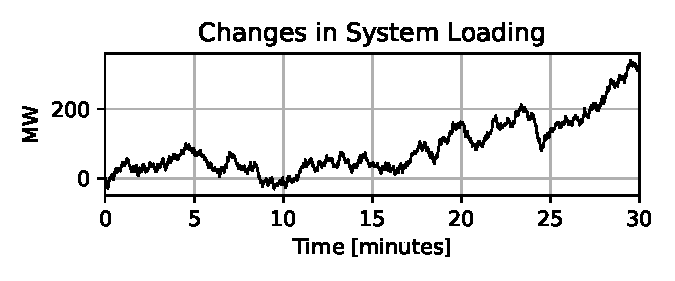
\includegraphics[width=\linewidth]{figures/miniWECCuniAccPloadChange}
\caption{Changes in total system loading.}
\label{fig: systemLoading}
\end{figure}

\begin{figure}[!ht]
\centering
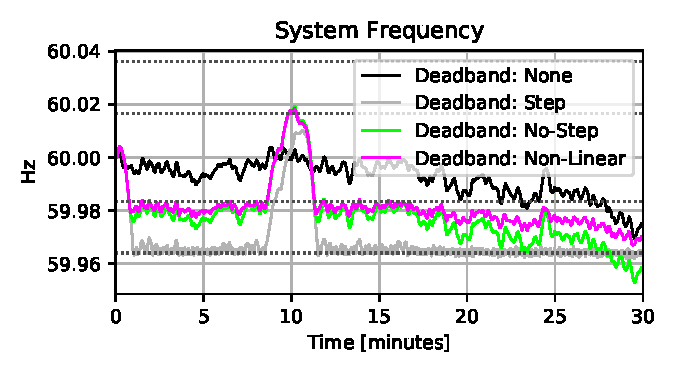
\includegraphics[width=\linewidth]{figures/miniWECCnoiseNLdroopDBFreq}
\caption{System frequency of various deadbands.}
\label{fig: sysFreqDB}
\end{figure}

The first three minutes of a single generators valve travel are shown in Fig. \ref{fig: valveComp} to compare how different deadbands affect movement.
A step deadband will send pulse train-esq control signals to the governor valve when system frequency is oscillating over the deadband. 
These repeated control pulses greatly increase valve travel over the more linear deadband options.
%The no-step deadband matches valve movement of the no deadband case after an initial delay.

\begin{figure}[!ht]
\centering
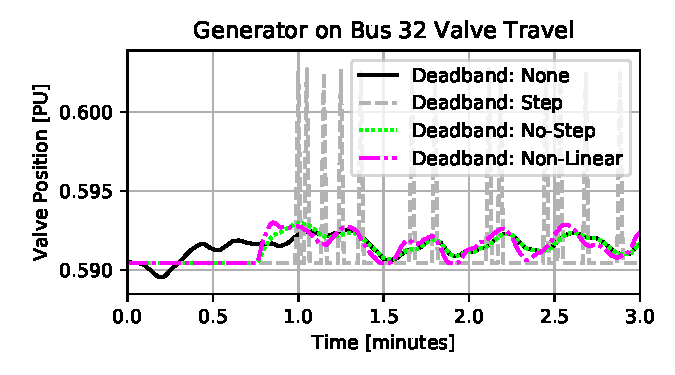
\includegraphics[width=\linewidth]{figures/gen32ValveComp}
\caption{Deadband valve movement comparisons.}
\label{fig: valveComp}
\end{figure}

Table \ref{tab: valveTravel} summarizes the valve travel for each generator in the system over the entire 30 minute simulation. A step type deadband has the largest total travel while the no deadband and no-step deadband cases are relatively similar.
The non-linear droop deadband has slightly more movement than the no-step case,.

% Testing of external table build for \input later
% Uses the IEEE table format guidelines
\begin{table}[!ht]
	\caption{Total valve travel for various deadband scenarios.}
	\label{tab: valveTravel}
	\centering
	\begin{tabular}{@{} C{1cm} S[table-format=2.2] S[table-format=2.2] S[table-format=2.2] S[table-format=2.2] S[table-format=2.2] @{}} 	
							\toprule							
		&	\multicolumn{5}{c}{Valve Travel [PU]}							\\	
	\text{Generator}	&	\text{No DB}	&	\text{Step}	&	\text{No-Step}	&	\text{\shortstack{N-L\\Droop}}  &	\text{\shortstack{No-Step\\Non-H}}	\\	\midrule	
	17	&	0.16	&	7.48	&	0.15	&	0.23	& 0.19 \\	
	23	&	0.16	&	7.48	&	0.15	&	0.23	& 0.19 \\	
	30	&	0.16	&	7.48	&	0.15	&	0.23	& 0.19 \\	
	32	&	0.16	&	7.54	&	0.15	&	0.23	& 0.19 \\	
	107	&	0.16	&	7.54	&	0.15	&	0.23	& 0.19 \\	
	41	&	0.15	&	6.44	&	0.14	&	0.23	& 0.06 \\	
	45	&	0.15	&	6.44	&	0.14	&	0.23	& 0.06 \\	
	53	&	0.16	&	7.54	&	0.15	&	0.23	& 0.06 \\	
	59	&	0.15	&	6.44	&	0.14	&	0.23	& 0.06 \\	\bottomrule
	Total:	&	1.41	&	64.38	&	1.32	&	2.07& 1.19 	\\	

	\end{tabular}

\end{table}


\subsection{Universal Acceptance Simulation Results}
To test partial acceptance of NERC deadband recommendations, all area deadbands were set to the no-step variety, but two of the three areas had a deadband of 16.6 mHz while the third was set to 36 mHz.
The resulting system frequency is shown in Fig. \ref{fig: uniFreq}.

\begin{figure}[!ht]
\centering
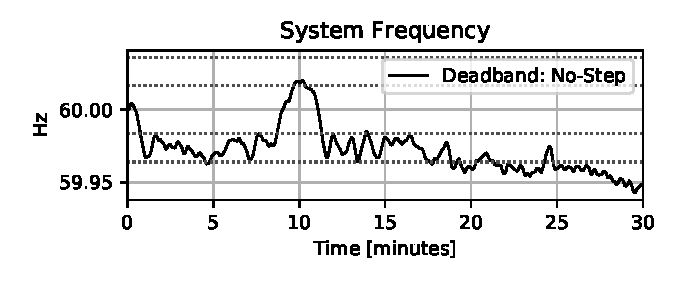
\includegraphics[width=\linewidth]{figures/miniWECCuniAccFreq}
\caption{System frequency to 0.03\% load noise of no-step deadbands with different area settings.}
\label{fig: uniFreq}
\end{figure}

As expected, Fig. \ref{fig: areaValveTravel} shows that the area with a larger deadband doesn't respond until after frequency drops below its deadband while the areas with smaller deadbands work to maintain frequency. 
Individual valve travel for each generator is shown in Table \ref{tab: valveTravel} under the `No-Step Alt DB' column.
In this case, the governor valves with a smaller deadband travel three times more than those with a larger deadband.

\begin{figure}[!ht]
\centering
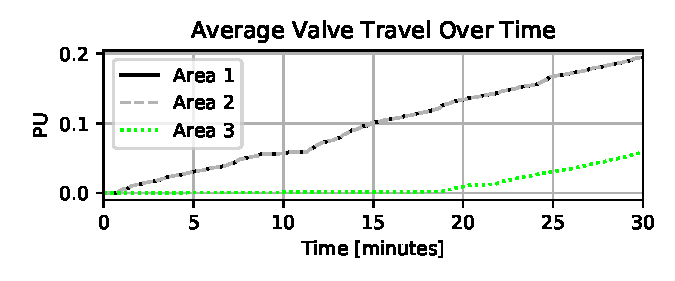
\includegraphics[width=\linewidth]{figures/miniWECCuniAccVTOverTime}
\caption{Average valve travel by area.}
\label{fig: areaValveTravel}
\end{figure}